\documentclass[12pt,a4paper]{article}
\usepackage[margin=2cm]{geometry}
\usepackage[T1]{fontenc}
\usepackage{lmodern}
\usepackage{setspace}
\usepackage{amsmath,amssymb,amsthm}
\usepackage{array}
\usepackage{booktabs}
\usepackage{longtable}
\usepackage{graphicx}
\usepackage[font=small,labelfont=bf]{caption}

\usepackage{tikz}
\usetikzlibrary{positioning,fit,backgrounds,arrows.meta}

\onehalfspacing

\begin{document}

\begin{titlepage}
\thispagestyle{empty}
\sffamily

\begin{center}
\vspace*{3.7cm}
{\Large School of Physics, Engineering and Technology}

\vspace{3.1cm}
{\fontsize{24}{28}\selectfont \textbf{BEng Project Initial Report}}

\vspace{1.3cm}
{\fontsize{22}{26}\selectfont \textbf{2025/6}}
\end{center}

\vfill
\noindent\textbf{Student Name:} Facundo Franchino

\vspace{1.2cm}
\noindent\textbf{Project Title:} Structured Riemannian Pruning of Feedback Delay Networks

\vspace{1.2cm}
\noindent\textbf{Supervisors:} Dr.\ Karolina Prawda

\end{titlepage}

\begin{abstract}
Artificial reverberation remains constrained by a persistent quality--efficiency gap. Measured Room Impulse Responses (RIRs) provide high acoustic fidelity, yet low-latency convolution is expensive when many long responses must be instantiated concurrently. Feedback Delay Networks (FDNs) offer a more attractive recursive alternative, but the acoustic smoothness required for colourless late reverberation increasingly favours very high orders, at which the dense feedback matrix introduces an $O(N^2)$ per-sample mixing bottleneck. This project investigates whether such massive, lossless FDNs can be systematically reduced to hardware-efficient structure without sacrificing either stability or perceptual quality.

A direct application of conventional unstructured pruning is unsuitable. In the lossless setting, the feedback matrix is constrained by $A^T A = I$, so arbitrary element removal generally violates the orthogonality constraint and destroys the very geometry that guarantees bounded energy. Moreover, the sparse patterns produced by magnitude pruning are poorly aligned with single-instruction multiple-data execution and cache-friendly memory access. 

The proposed solution is therefore not to prune entries independently. Instead,
the project starts from a dense lossless reference operator, either learned
through FLAMO's implicit orthogonal parameterisation or specified directly at
high order, and then projects it onto a structured feasible subset centred on
block-circulant topology. The reduction step is guided by ranking criteria
derived from temporal activations and perceptually weighted response error
rather than raw coefficient magnitude.

The resulting structure will be exported as a deployment blueprint and realised
as a custom C++ inference node using RTNeural-style real-time design and AVX2
vectorisation. The longer-term goal is to convert dense differentiable FDNs into
real-time viable reverberation engines.
\end{abstract}

\clearpage

\section{Introduction and Aims}

\paragraph{Aim.}
The aim of this project is to develop and evaluate a structured pruning method
for dense lossless Feedback Delay Networks, such that acoustically effective
high-order designs can be reduced to computationally efficient real-time forms
without unacceptable loss of stability or sound quality.




\paragraph{Objectives.}
To support this aim, the project has four objectives:
\begin{enumerate}
    \item construct dense lossless FDN reference systems for high-order diffusion and RIR-matching scenarios, and verify their baseline acoustic behaviour and stability;
    \item develop at least one structured reduction method for mapping dense feedback operators onto a computationally efficient topology, and quantify the resulting structural and orthogonality error;
    \item compare magnitude-, activation-, and perceptually guided reduction criteria using defined acoustic and computational metrics;
    \item implement a real-time C++ prototype of the structured design and benchmark it against the dense baseline in terms of runtime, memory footprint, orthogonality defect or approximation error, and acoustic deviation.
\end{enumerate}






\begin{figure}[t]
    \centering
    % \makebox allows the figure to be wider than the text margins without throwing an error
    \makebox[\textwidth][c]{
    \resizebox{1.15\textwidth}{!}{
    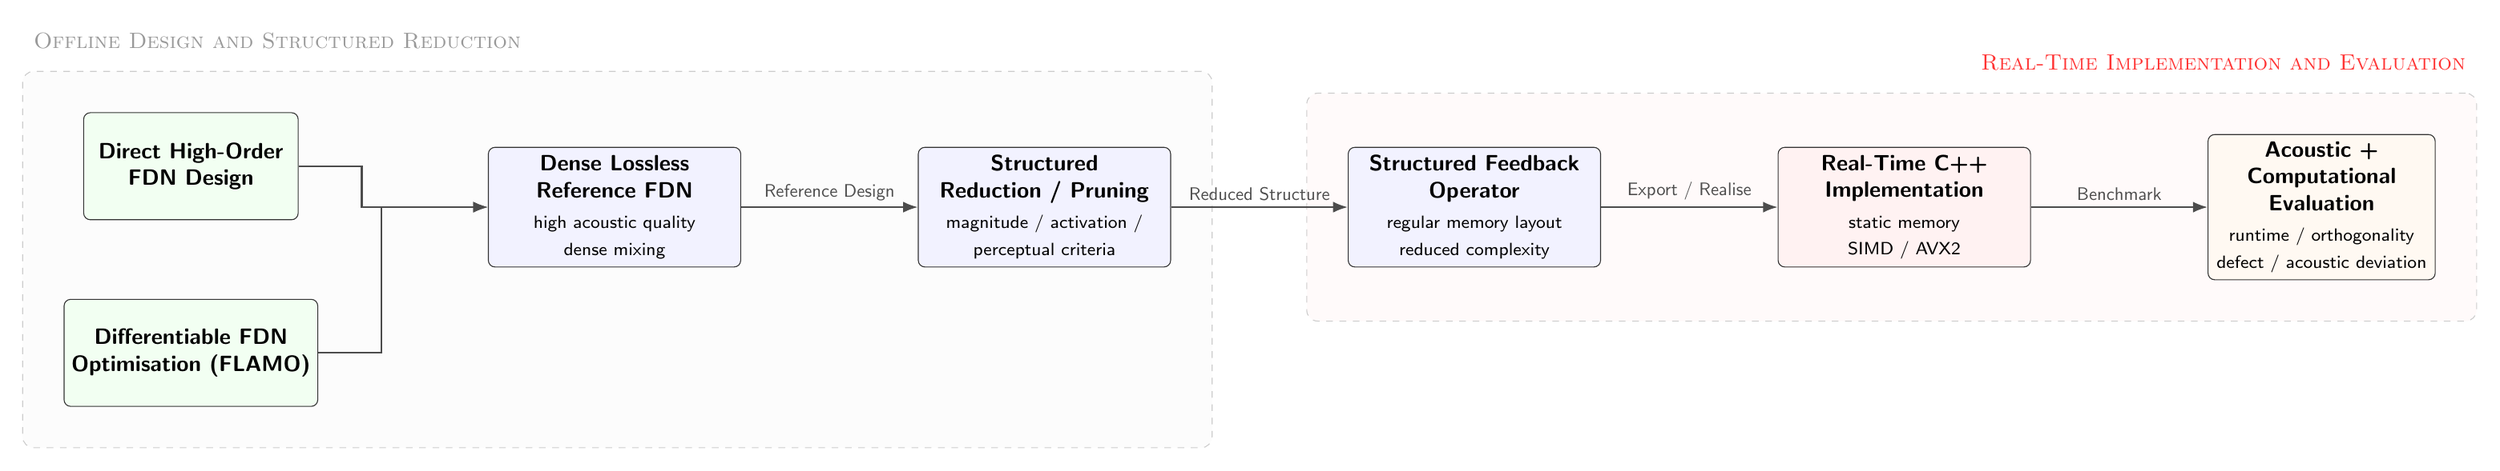
\begin{tikzpicture}[
        node distance=1.8cm and 2.3cm,
        font=\sffamily,
        process/.style={rectangle, minimum width=4.0cm, minimum height=1.9cm, text centered, draw=black!80, fill=blue!5, rounded corners=3pt, align=center},
        data/.style={rectangle, minimum width=3.4cm, minimum height=1.7cm, text centered, draw=black!80, fill=green!5, rounded corners=3pt, align=center},
        evalbox/.style={rectangle, minimum width=3.6cm, minimum height=1.9cm, text centered, draw=black!80, fill=orange!5, rounded corners=3pt, align=center},
        arrow/.style={thick, ->, >=Latex, color=black!70},
        groupbox/.style={draw=gray!40, dashed, inner sep=0.65cm, rounded corners=5pt, fill=gray!2}
    ]

        % --- Input routes ---
        \node (input1) [data] {\textbf{Direct High-Order}\\\textbf{FDN Design}};
        \node (input2) [data, below=1.25cm of input1] {\textbf{Differentiable FDN}\\\textbf{Optimisation (FLAMO)}};

        % --- Dense reference ---
        \node (dense) [process, right=3.0cm of input1, yshift=-0.65cm] {\textbf{Dense Lossless}\\\textbf{Reference FDN}\\[2pt]
        \footnotesize high acoustic quality\\
        \footnotesize dense mixing};

        % --- Structured reduction ---
        \node (prune) [process, right=2.8cm of dense] {\textbf{Structured}\\\textbf{Reduction / Pruning}\\[2pt]
        \footnotesize magnitude / activation /\\
        \footnotesize perceptual criteria};

        % --- Structured operator ---
        \node (struct) [process, right=2.8cm of prune] {\textbf{Structured Feedback}\\\textbf{Operator}\\[2pt]
        \footnotesize regular memory layout\\
        \footnotesize reduced complexity};

        % --- Deployment ---
        \node (deploy) [process, right=2.8cm of struct, fill=red!5] {\textbf{Real-Time C++}\\\textbf{Implementation}\\[2pt]
        \footnotesize static memory\\
        \footnotesize SIMD / AVX2};

        % --- Evaluation ---
        \node (eval) [evalbox, right=2.8cm of deploy] {\textbf{Acoustic +}\\\textbf{Computational}\\\textbf{Evaluation}\\[2pt]
        \footnotesize runtime / orthogonality\\
        \footnotesize defect / acoustic deviation};

        % --- Connections ---
        \draw [arrow] (input1.east) -- ++(1.0cm,0) |- (dense.west);
        \draw [arrow] (input2.east) -- ++(1.0cm,0) |- (dense.west);

        \draw [arrow] (dense) -- node[above, scale=0.82] {Reference Design} (prune);
        \draw [arrow] (prune) -- node[above, scale=0.82] {Reduced Structure} (struct);
        \draw [arrow] (struct) -- node[above, scale=0.82] {Export / Realise} (deploy);
        \draw [arrow] (deploy) -- node[above, scale=0.82] {Benchmark} (eval);

        % --- Grouping boxes ---
        \begin{scope}[on background layer]
            \node (offlinebox) [groupbox,
                fit=(input1) (input2) (dense) (prune),
                label={[anchor=south west, inner sep=5pt, text=gray!80, yshift=5pt]north west:\textsc{Offline Design and Structured Reduction}}
            ] {};
        \end{scope}

        \begin{scope}[on background layer]
            \node (rtbox) [groupbox,
                fit=(struct) (deploy) (eval),
                fill=red!2,
                label={[anchor=south east, inner sep=5pt, text=red!80, yshift=5pt]north east:\textsc{Real-Time Implementation and Evaluation}}
            ] {};
        \end{scope}

    \end{tikzpicture}
    }
    }
    % \footnotesize added here to shrink the caption text
    \caption{\footnotesize Overall project pipeline. A dense acoustically effective FDN is first obtained either by direct high-order construction or by differentiable optimisation in FLAMO, then reduced to a structured form and finally evaluated in real-time implementation.}
    \label{fig:pipeline}
\end{figure}








Artificial reverberation has long been shaped by a fundamental trade-off between
acoustic realism and computational efficiency, often described in digital signal
processing (DSP) as the quality-efficiency gap. At one end of this continuum,
convolution with measured Room Impulse Responses (RIRs) provides a highly faithful
representation of a physical space. However, the need to process long sample
sequences results in a complexity that scales as $O(L \log L)$, where $L$ denotes
the impulse-response length. Even when fast convolution methods are employed,
the associated memory traffic, buffering overhead, and latency penalties remain
substantial, making convolution computationally prohibitive for multiple concurrent
instances under low-latency real-time constraints on consumer-grade central
processing units (CPUs).

By contrast, algorithmic reverberators, most notably Feedback Delay Networks
(FDNs), offer computationally efficient recursive structures whose per-sample cost
scales approximately linearly with the number of delay lines, $N$. In such systems,
reverberation is generated not by direct reproduction of a measured impulse response,
but through recirculation within a network of delay lines coupled by a feedback
matrix. This architecture has made FDNs one of the most influential formulations
in algorithmic reverberation, since they provide a favourable balance between
computational efficiency, parametric flexibility, and perceptual plausibility.
Yet traditional low-order FDNs, typically based on $4 \times 4$ or $8 \times 8$
feedback matrices, often exhibit insufficient modal density. The resulting sparsity
of resonant modes gives rise to metallic coloration and audible ringing artefacts,
since the auditory system can resolve individual resonances that do not blend into
a diffuse statistical sound field.

A natural response is therefore to increase the order of the network. In principle,
high-order FDNs can produce denser mode distributions, faster echo build-up, and
more nearly diffuse late reverberation. However, this improvement is not obtained
without cost. If the feedback matrix is dense, the mixing stage scales quadratically,
so that the per-sample cost of matrix-vector multiplication becomes $O(N^2)$.
For sufficiently large networks, this mixer dominates the computational budget,
even if the delay lines themselves remain inexpensive. The central difficulty is
thus to retain the acoustic benefits of high-order, lossless mixing without
inheriting the full computational cost of a dense feedback operator. In
practical terms, the project asks whether a large artificial reverberator that
already sounds good can be simplified into a much faster structure without
losing too much of its acoustic character.

This project argues that the appropriate response to this difficulty is not merely
better optimisation, but structured pruning. In the present context, pruning
denotes the systematic reduction of a dense Feedback Delay Network into a
computationally efficient structured form by removing, constraining, or
reorganising degrees of freedom in its feedback matrix while preserving, as far
as possible, the stability, diffuseness, and acoustic behaviour of the original
design. Although pruning is well established in neural-network compression as a
means of reducing computational cost while retaining useful global behaviour, it
has not become a standard design principle for Feedback Delay Networks. The
present work therefore examines whether that idea can be reformulated for
artificial reverberation, where the objects being pruned are not arbitrary
parameter arrays but lossless feedback operators subject to geometric,
dynamical, and perceptual constraints.

The intended contribution of the project is a structured, geometry-aware
reduction method for dense lossless Feedback Delay Networks, that is, for
reducing dense feedback structures while respecting the geometry that keeps them
stable. The term
\emph{Riemannian} is essential here because the feedback matrices of
interest must remain within constrained classes such as orthogonal or otherwise
lossless operators. Pruning therefore cannot be treated as unconstrained
coefficient removal alone. Instead, the reduction process must respect the geometry
of the feasible set. The novelty of the work lies not simply in applying
manifold-aware optimisation to FDNs, nor simply in borrowing pruning language
from machine learning, but in combining the two into a single methodology for
converting dense, acoustically effective FDNs into efficient structured real-time
systems.

Two application settings motivate this framework. The first is the construction
of extremely high-order FDNs, for example with $N=1024$ or $N=4096$, whose dense
mixing would otherwise be too expensive for practical use. In this regime, the
goal of pruning is to preserve the diffuse, high-modal-density behaviour needed
to suppress metallic artefacts while approaching the efficiency of fast
structured transforms. The second is the deployment of differentiable
reverberators, particularly in frameworks such as FLAMO, where dense orthogonal
feedback matrices may be optimised to mimic a target Room Impulse Response. In
that setting, pruning is intended to transform a learned but computationally
heavy FDN into a real-time implementable structure while preserving acoustic
fidelity to the reference RIR.



For an electronic engineer, the essential point is simple: a lossless feedback
matrix cannot be edited coefficient by coefficient in the same way as an
ordinary unconstrained gain matrix, because its entries are coupled by the
energy-preserving condition.

\subsection{Why the feedback matrix is a geometric object}

For a real-valued lossless FDN, the feedback matrix must preserve
Euclidean energy, and therefore satisfy
\[
A^T A = I.
\]
The feasible set is therefore not the full ambient space
$\mathbb{R}^{N \times N}$ but the orthogonal group $O(N)$, i.e.\ the square
case of the Stiefel manifold \cite{boumal}. This has an immediate engineering
consequence: once orthogonality is imposed, the coefficients are no longer free
to vary independently. Admissible perturbations must satisfy
\[
X^T V + V^T X = 0,
\]
so the degrees of freedom are coupled by the constraint itself \cite{boumal}.

This coupling matters directly for pruning. If the feedback matrix
is treated as just a table of coefficients, then deleting or modifying
individual entries appears harmless. Geometrically, however, such
edits generally leave the feasible set immediately. In this setting,
pruning cannot be understood as independent coefficient removal.
The feedback matrix is a geometric object, and any principled
reduction procedure must respect that geometry \cite{boumal}.

\subsection{Why unstructured magnitude pruning fails in this setting}

In neural-network pruning, the canonical baseline is iterative
magnitude pruning. This consists of training a dense model, removing the parameters of
smallest magnitude, and optionally retraining the surviving
subnetwork \cite{frankle}. This idea is historically important
and often empirically effective in over-parameterised learning
systems. It is therefore a natural point of comparison. However,
the assumptions that make magnitude pruning plausible in generic
neural networks do not transfer cleanly to lossless FDN mixing.

The first difficulty is geometric. In an orthogonal feedback matrix,
coefficient values are not independently meaningful in the usual
way, because row and column norms are globally constrained.
Magnitude is therefore a poor proxy for importance. In canonical
dense orthogonal constructions such as the normalised Hadamard
matrix, every entry has identical magnitude $1/\sqrt{N}$, so there
is no intrinsic population of ``small'' coefficients to remove. More
generally, even when magnitudes are unequal, the effect of a single
coefficient is mediated by the orthogonality of the whole operator.
Removing one entry does not merely delete a weak connection; it
perturbs a balance condition shared by the corresponding row and
column.

The second difficulty is feasibility. If $A$ is orthogonal and one forms a masked matrix
$\tilde{A} = A \odot M$, with $M$ a binary mask, then in general
$\tilde{A}^T \tilde{A} \neq I$.

Figure~\ref{fig:pruningbreaksorthogonality} illustrates schematically why arbitrary entrywise pruning breaks the lossless constraint.

\begin{figure}[t]
    \centering
    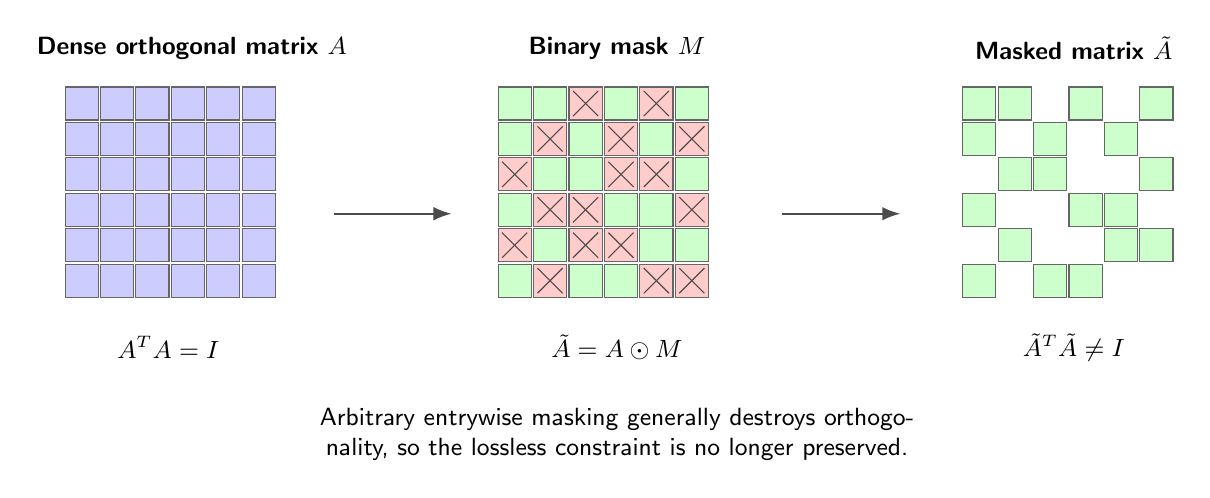
\begin{tikzpicture}[
        font=\sffamily,
        cell/.style={draw=black!60, minimum width=0.42cm, minimum height=0.42cm, inner sep=0pt},
        filled/.style={cell, fill=blue!20},
        kept/.style={cell, fill=green!20},
        pruned/.style={cell, fill=red!20},
        labelstyle/.style={align=center, font=\sffamily\small},
        arrow/.style={thick, ->, >=Latex, color=black!70}
    ]

    % --- Panel titles ---
    \node[labelstyle] at (1.4,1.9) {\textbf{Dense orthogonal matrix $A$}};
    \node[labelstyle] at (6.8,1.9) {\textbf{Binary mask $M$}};
    \node[labelstyle] at (12.6,1.9) {\textbf{Masked matrix $\tilde{A}$}};

    % --- Panel 1: Dense orthogonal matrix A ---
    \foreach \i in {0,...,5} {
        \foreach \j in {0,...,5} {
            \node[filled] at (\j*0.45, 1.2-\i*0.45) {};
        }
    }
    \node[labelstyle] at (1.1,-1.9) {$A^T A = I$};

    % --- Arrow 1 ---
    \draw[arrow] (3.2,-0.2) -- (4.7,-0.2);

    % --- Panel 2: Binary mask M ---
    \foreach \i/\j in {
        0/0,0/1,0/3,0/5,
        1/0,1/2,1/4,
        2/1,2/2,2/5,
        3/0,3/3,3/4,
        4/1,4/4,4/5,
        5/0,5/2,5/3
    } {
        \node[kept] at (5.5+\j*0.45, 1.2-\i*0.45) {};
    }

    \foreach \i/\j in {
        0/2,0/4,
        1/1,1/3,1/5,
        2/0,2/3,2/4,
        3/1,3/2,3/5,
        4/0,4/2,4/3,
        5/1,5/4,5/5
    } {
        \node[pruned] at (5.5+\j*0.45, 1.2-\i*0.45) {};
        \draw[black!70] (5.5+\j*0.45-0.16, 1.2-\i*0.45-0.16) -- (5.5+\j*0.45+0.16, 1.2-\i*0.45+0.16);
        \draw[black!70] (5.5+\j*0.45-0.16, 1.2-\i*0.45+0.16) -- (5.5+\j*0.45+0.16, 1.2-\i*0.45-0.16);
    }

    \node[labelstyle] at (6.8,-1.9) {$\tilde{A} = A \odot M$};

    % --- Arrow 2 ---
    \draw[arrow] (8.9,-0.2) -- (10.4,-0.2);

    % --- Panel 3: Masked matrix A~ ---
    \foreach \i/\j in {
        0/0,0/1,0/3,0/5,
        1/0,1/2,1/4,
        2/1,2/2,2/5,
        3/0,3/3,3/4,
        4/1,4/4,4/5,
        5/0,5/2,5/3
    } {
        \node[kept] at (11.4+\j*0.45, 1.2-\i*0.45) {};
    }

    \node[labelstyle] at (12.6,-1.9) {$\tilde{A}^T \tilde{A} \neq I$};

    % --- Bottom note ---
    \node[labelstyle, text width=11.5cm] at (6.8,-3.0)
    {Arbitrary entrywise masking generally destroys orthogonality, so the lossless constraint is no longer preserved.};

    \end{tikzpicture}
    \caption{Schematic illustration of why naive entrywise pruning fails for lossless feedback matrices. Arbitrary masking of an orthogonal matrix generally destroys the orthogonality condition and therefore breaks the lossless constraint.}
    \label{fig:pruningbreaksorthogonality}
\end{figure}




The lossless property is therefore destroyed by arbitrary entrywise
pruning. Any subsequent attempt to restore orthogonality must
include some projection or reparameterisation step, at which point
the original unstructured pruning decision has already been altered.
In other words, naïve sparsification and geometric feasibility are in
tension from the outset.

The third difficulty is computational rather than geometric.
Unstructured sparsity is not automatically fast. Clarke and
Chowdhury point out that sparse matrix multiplies often rely on
indirect memory accesses, and that this is especially problematic in
real-time audio, where efficient inference depends heavily on
hardware-level primitives requiring sequential memory access, such
as SIMD operations \cite{clarke}. This observation
is highly relevant here. Even if approximate orthogonality could be
maintained under entrywise pruning, the resulting sparsity pattern
would still be poorly aligned with the requirements of
vectorisation-friendly CPU inference.

For these reasons, unstructured magnitude pruning is best treated
here as a useful contrast case rather than as the main design
principle. Frankle clarifies why it became the dominant pruning
baseline in machine learning \cite{frankle}; Boumal explains
why orthogonality couples the coefficients globally
\cite{boumal}; and Clarke and Chowdhury show why
inference-time efficiency depends on structured memory layout
rather than sparsity alone \cite{clarke}. Taken
together, these observations justify the shift from unstructured
magnitude pruning toward structured, geometry-aware reduction.

At an engineering level, this becomes a question of implementation: should the
orthogonality constraint be enforced directly during optimisation, or built into
the parameterisation from the outset?

\subsection{Implicit versus explicit manifold optimisation}

From a geometric point of view, direct optimisation on $O(N)$ is
perfectly natural \cite{boumal}. However, the training phase need
not be implemented in that explicit form. FLAMO already provides a
differentiable environment for frequency-domain optimisation of
linear time-invariant audio systems within PyTorch, including
orthogonality-preserving matrix parameterisations \cite{flamo}. In
its FDN case study, the feedback matrix is implemented as a learnable
matrix with orthogonal mapping, allowing the optimisation of a
lossless FDN directly within the differentiable framework
\cite{flamo}.

For the present project, this makes FLAMO the practical training
vehicle. Boumal remains the right source for understanding the
geometry of the feasible set \cite{boumal}, whereas FLAMO provides
an implementation pathway for training dense lossless FDNs inside an
autodiff system \cite{flamo}. Thus explicit manifold optimisation
remains conceptually central, even if the optimisation procedure is
carried out through an implicit orthogonality-preserving
parameterisation.

\subsection{Differentiable DSP and deployment tension}

The broader context for this project is differentiable digital signal
processing. DDSP argues for combining classic signal-processing
structure with automatic differentiation, so that strong inductive
biases and interpretable modules can be retained without giving up
the expressive advantages of neural learning
\cite{ddsp}. FLAMO extends this general philosophy to
frequency-domain optimisation of differentiable LTI audio modules,
including reverberation structures \cite{flamo}. This
makes it natural to learn a dense, acoustically meaningful FDN in a
differentiable environment before asking how it should be deployed.

The deployment problem is governed by a different set of
constraints. Training favours flexible tensor abstractions, rich
parameterisations, and batch-oriented computation. Real-time audio
does not. RTNeural makes this distinction especially clear. In hard
real-time systems, one must avoid unbounded-time operations in the
audio thread, including memory allocation, thread locking, garbage
collection, and similar mechanisms \cite{chowdhury}.
The same paper argues that, for the small models typical of
real-time use, CPU inference with SIMD support is often as fast
as or faster than GPU execution, precisely because it avoids the
overheads that real-time systems cannot tolerate
\cite{chowdhury}. Its compile-time API is relevant
for the same reason: memory is allocated statically, functions may
be inlined, and loops can be unrolled when dimensions are known
at compile time \cite{chowdhury}.

Although RTNeural is a neural inference library rather than an FDN
library, the deployment lesson transfers directly. A real-time FDN
implementation should favour fixed dimensions where possible,
pre-allocated buffers, contiguous memory, bounded-time
operations, and arithmetic that is friendly to SIMD
vectorisation. This is precisely why structured pruning matters in
the present setting. The goal is not only to reduce parameter count
in an abstract sense, but to transform a dense differentiably trained
FDN into a form whose topology is compatible with real-time CPU
execution.

\subsection{Critical synthesis}

The literature therefore points toward a fairly specific
methodological direction. Boumal provides the geometric language
needed to formulate the feedback matrix as a constrained object on
the orthogonal group rather than as an unconstrained parameter
array \cite{boumal}. Frankle provides the historical and
methodological background for pruning, particularly the role of
magnitude pruning as a dominant baseline in neural-network
compression \cite{frankle}. Clarke and Chowdhury shift that
discussion toward inference-time structure, showing that the
difference between sparsity and speed is especially important in
real-time audio \cite{clarke}. DDSP supplies the
broader differentiable-signal-processing rationale
\cite{ddsp}, FLAMO provides a practical framework for
training dense orthogonality-constrained FDNs
\cite{flamo}, and RTNeural clarifies the systems-level
discipline required for deployable real-time C++ implementations
\cite{chowdhury}.

Taken together, the literature motivates the present project. None of the cited
sources provides a complete procedure for taking a dense, acoustically effective,
lossless FDN and converting it into a structured real-time implementation
without unacceptable acoustic loss.

\section{Intended Approach and Methodology}

The methodology is organised as a three-phase pipeline that moves from dense
reference construction to structured reduction and finally to real-time
deployment.

\subsection{Phase 1: construction of the dense reference system}

The first phase constructs the dense FDN reference system against which later
structured reductions will be judged. Two use-cases are considered. The first
is a high-order diffuse late-reverberation setting, in which a large lossless
FDN is specified directly and treated as the acoustic reference object. The
second is an RIR-matching setting, in which a differentiable FDN is optimised
in FLAMO to approximate a target room response. In both cases, the aim is to
begin from a dense acoustically effective reference before introducing
computational structure.

This phase is intentionally dense. Its purpose is to separate acoustical
design from computational simplification. If structure is imposed too
early, it becomes difficult to determine whether a failure is due to limited
topology or inadequate training. The dense reference therefore serves as an
upper bound on the quality attainable under the chosen loss, optimisation
procedure, and parameterisation.

The output of this phase is a dense reference feedback operator
$A_{\mathrm{dense}}$, together with the associated delay and attenuation
parameters. Additional analysis will include echo-density profiles,
spectrograms, and, where applicable, deviation from the target response.

\subsection{Phase 2: structured projection and psychoacoustic ranking}

The second phase forms the scientific core of the project. Here, a dense
orthogonal solution is reduced to a structured feasible subset. Block-circulant
structure is the primary candidate, since it offers regular memory layout and
admits fast multiplication through smaller transform-like operations.






Figure~\ref{fig:densevsstructuredfdn} shows the conceptual transition from dense high-order mixing to a structured reduced topology.




\begin{figure}[t]
    \centering
    \makebox[\textwidth][c]{
    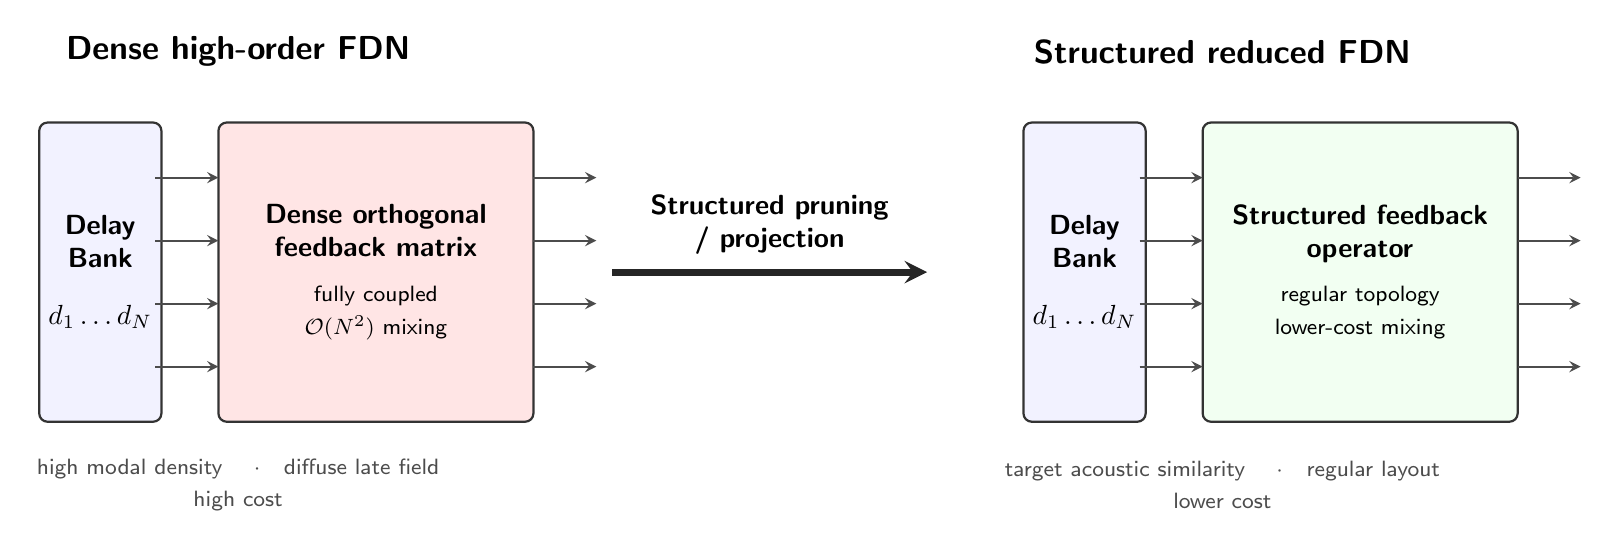
\begin{tikzpicture}[
        font=\sffamily,
        >=stealth,
        % Styles
        delaybank/.style={rectangle, draw=black!80, thick, fill=blue!5, minimum width=1.4cm, minimum height=3.8cm, align=center, rounded corners=3pt},
        densemat/.style={rectangle, draw=black!80, thick, fill=red!10, minimum width=4.0cm, minimum height=3.8cm, align=center, rounded corners=3pt},
        structmat/.style={rectangle, draw=black!80, thick, fill=green!5, minimum width=4.0cm, minimum height=3.8cm, align=center, rounded corners=3pt},
        title/.style={font=\sffamily\bfseries\large},
        % Shrunk font size and tight line spacing for the bottom notes
        note/.style={font=\sffamily\footnotesize, align=center, text=black!70}, 
        arrow/.style={thick, ->, color=black!70}
    ]

    % ================= LEFT PANEL =================
    \node[title] at (1.75, 2.8) {Dense high-order FDN};

    % Delay Bank
    \node[delaybank] (dleft) at (0, 0) {\textbf{Delay}\\\textbf{Bank}\\[3mm] $d_1 \dots d_N$};
    
    % Dense Matrix
    \node[densemat] (mleft) at (3.5, 0) {\textbf{Dense orthogonal}\\\textbf{feedback matrix}\\[4pt] \footnotesize fully coupled \\ \footnotesize $\mathcal{O}(N^2)$ mixing};

    % Connections Left 
    \foreach \y in {1.2, 0.4, -0.4, -1.2} {
        \draw[arrow] (0.7, \y) -- (1.5, \y);
        \draw[arrow] (5.5, \y) -- (6.3, \y);
    }

    % Notes Left - Stacked to pull less horizontal weight
    \node[note] at (1.75, -2.7) {high modal density \quad$\cdot$\quad diffuse late field\\[2pt] high cost};


    % ================= MIDDLE ARROW =================
    % Thicker line width and darker color to make it the visual anchor
    \draw[-{stealth}, color=black!85, line width=2.5pt] (6.5, 0) -- (10.5, 0);
    \node[align=center, font=\sffamily\bfseries] at (8.5, 0.6) {Structured pruning \\ / projection};


    % ================= RIGHT PANEL =================
    \node[title] at (14.25, 2.8) {Structured reduced FDN};

    % Delay Bank 
    \node[delaybank] (dright) at (12.5, 0) {\textbf{Delay}\\\textbf{Bank}\\[3mm] $d_1 \dots d_N$};
    
    % Structured Matrix (Sub-blocks removed, text placed directly inside)
    \node[structmat] (mright) at (16.0, 0) {\textbf{Structured feedback}\\\textbf{operator}\\[4pt] \footnotesize regular topology \\ \footnotesize lower-cost mixing};

    % Connections Right
    \foreach \y in {1.2, 0.4, -0.4, -1.2} {
        \draw[arrow] (13.2, \y) -- (14.0, \y);
        \draw[arrow] (18.0, \y) -- (18.8, \y);
    }

    % Notes Right - Stacked to pull less horizontal weight
    \node[note] at (14.25, -2.7) {target acoustic similarity \quad$\cdot$\quad regular layout\\[2pt] lower cost};

    \end{tikzpicture}
    }
    \caption{Conceptual transition from a dense high-order FDN to a structured reduced FDN.}
    \label{fig:densevsstructuredfdn}
\end{figure}





At a high level, if
$A_{\mathrm{dense}}$ denotes the learned reference, the structured problem is
\[
A_{\mathrm{struct}} = \arg\min_{A \in \mathcal{S}} \mathcal{J}(A;A_{\mathrm{dense}}),
\]
where $\mathcal{S}$ denotes a structured feasible set, ideally intersecting the
orthogonal group or else approximating it closely, and $\mathcal{J}$ measures
functional and acoustic deviation.

Three ranking principles will be compared.

\textbf{(i) Magnitude baseline.}
This is included only as a control. It follows the conventional idea of removing
small coefficients or small structural blocks, and is expected to perform poorly
for the geometric and computational reasons established earlier.

\textbf{(ii) Temporal mean activations.}
Inspired by Clarke and Chowdhury's activation-based ranking, the FDN will be
driven by representative signals and its internal state trajectories will be
analysed. Delay-line couplings or structural blocks whose removal induces only a
small change in average propagated activation energy will receive low
importance scores. The point is to infer importance from dynamical
participation rather than from static coefficient magnitude.

\textbf{(iii) Perceptually weighted response error.}
A third ranking criterion will be explored based on the deviation between the
dense and structured FDN responses in a perceptually weighted time-frequency
representation. The guiding idea is that pruning decisions should be judged not
only by coefficient values or internal activations, but also by their effect on
acoustically salient properties such as early echo build-up, decay smoothness,
and spectral coloration. This criterion is exploratory, and its precise form
remains part of the methodological development of the project.

The projection itself may be implemented in stages. One possibility is block
selection followed by orthogonal re-fitting within the retained topology.
Another is alternating minimisation between a structural mask and a subsequent
re-orthogonalisation or structured factorisation step. If exact orthogonality cannot be maintained within the chosen topology, the
report will distinguish clearly between exact feasible reduction and approximate
reduction. The deviation will then be quantified through metrics such as
$\|A^T A - I\|_F$ alongside the acoustic criteria. This distinction matters,
because the term ``submanifold'' is justified only when the feasible set is
smooth and closed under the chosen parameterisation; some structured subsets may
instead be better understood as discrete topologies equipped with local
continuous parameters.

\subsection{Phase 3: JSON export and real-time C++ realisation}

Once a structured model has been obtained, the final phase concerns deployment.
Following the general workflow used in RTNeural, the trained or projected
parameters will be exported as a compact blueprint, for example in JSON form,
and used to instantiate a custom C++ block-circulant node. The implementation
will be designed around hard real-time constraints: no dynamic allocation in the
audio thread, fixed-size or pre-allocated buffers, contiguous block storage,
AVX2-aware vectorised inner loops, and reproducible benchmarking against the
dense baseline.

The target computational improvement is to replace naive dense mixing with a
structure approaching $O(N \log N)$ arithmetic cost, or at least to achieve a
substantially lower constant factor through regular block reuse and
vectorisation. That asymptotic claim must, however, be interpreted carefully.
It is valid only if the selected structure genuinely admits fast transform-based
multiplication. If the final feasible subset deviates from pure circulant
algebra, the project will report the measured complexity and cycle counts
directly rather than retaining the asymptotic claim by assumption.

Evaluation in this phase will include wall-clock real-time factor, per-block
processing time, memory footprint, orthogonality defect where relevant, and
acoustic deviation from the dense reference.

In practical terms, the minimum successful outcome of the project will be a
working structured reduction and C++ implementation for at least one dense
reference FDN, together with quantitative comparison against the dense baseline.
The evaluation will focus primarily on FDN orders in the range $N=64$ to
$N=1024$, with higher orders explored if time permits. A meaningful result would
consist of a measurable runtime reduction relative to dense mixing, bounded
orthogonality defect or clearly reported approximation error, and no severe
reintroduction of metallic artefacts in the reduced design. If the block-circulant
route proves too restrictive, the fallback deliverable will be a structured
approximation method with explicit trade-off analysis rather than exact
manifold-preserving reduction.

Figure~\ref{fig:tradeoff} summarises the three-way trade-off that governs the evaluation of structured FDN reduction.




\begin{figure}[t]
    \centering
    \makebox[\textwidth][c]{
    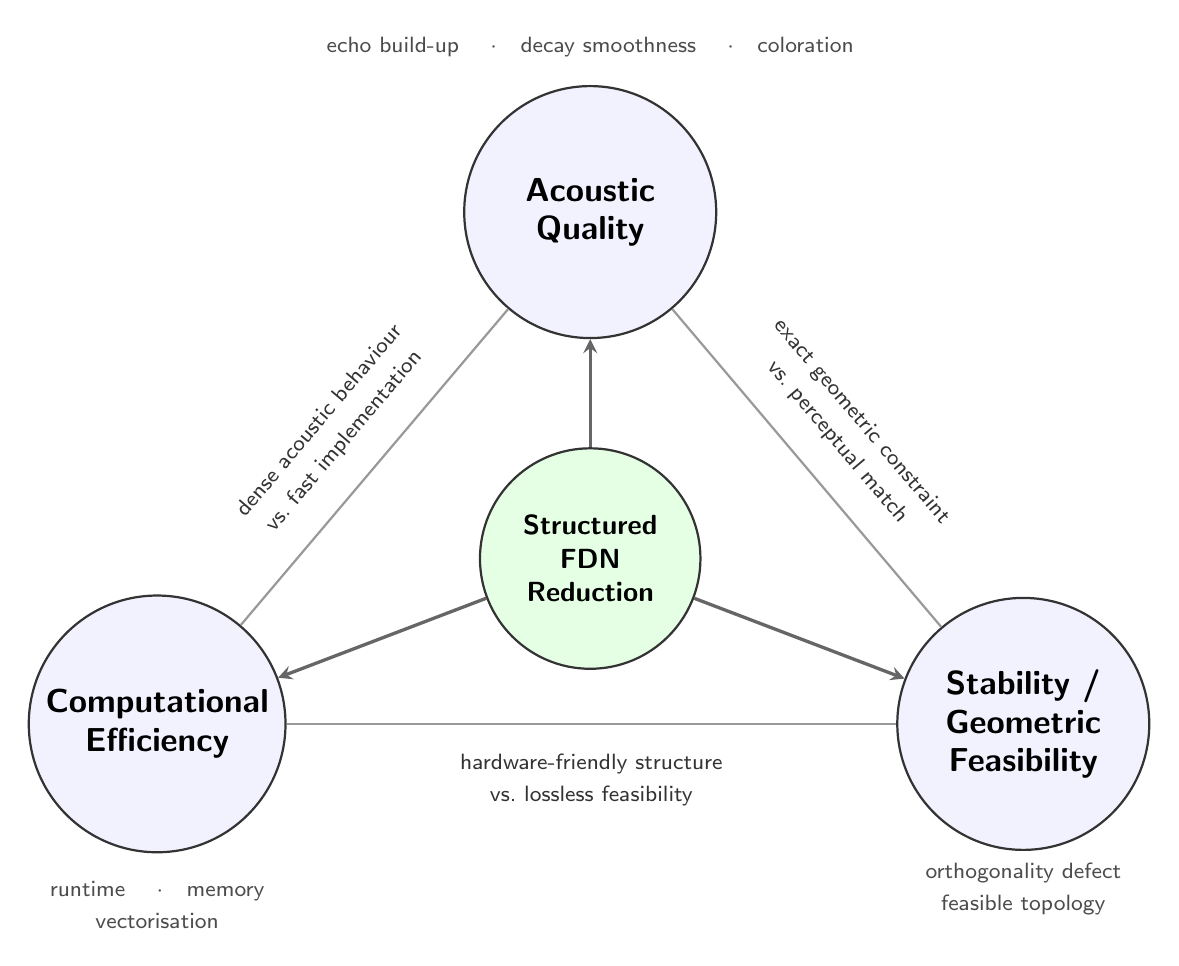
\begin{tikzpicture}[
        font=\sffamily,
        >=stealth,
        % Styles
        vertex/.style={circle, draw=black!80, thick, fill=blue!5, minimum size=3.2cm, align=center, font=\sffamily\bfseries\large},
        centerbox/.style={circle, draw=black!80, thick, fill=green!10, minimum size=2.8cm, align=center, font=\sffamily\bfseries},
        edgelabel/.style={font=\sffamily\footnotesize, align=center, text=black!80},
        note/.style={font=\sffamily\footnotesize, align=center, text=black!70},
        tri/.style={thick, color=black!40},
        innerarrow/.style={thick, ->, color=black!60, line width=1.2pt}
    ]

    % ================= MAIN NODES =================
    \node[vertex] (acoustic) at (0, 6.5) {Acoustic\\Quality};
    \node[vertex] (efficiency) at (-5.5, 0) {Computational\\Efficiency};
    \node[vertex] (geometry) at (5.5, 0) {Stability /\\Geometric\\Feasibility};

    % ================= TRIANGLE EDGES =================
    % Drawn between the borders of the nodes. 
    % Labels are 'sloped' to follow the line angle and pushed 'above' or 'below' to sit outside the triangle.
    \draw[tri] (efficiency) -- node[midway, edgelabel, sloped, above=0.25cm] {dense acoustic behaviour\\[2pt]vs.\ fast implementation} (acoustic);
    \draw[tri] (acoustic) -- node[midway, edgelabel, sloped, above=0.25cm] {exact geometric constraint\\[2pt]vs.\ perceptual match} (geometry);
    \draw[tri] (efficiency) -- node[midway, edgelabel, below=0.25cm] {hardware-friendly structure\\[2pt]vs.\ lossless feasibility} (geometry);

    % ================= CENTER NODE =================
    \node[centerbox] (center) at (0, 2.1) {Structured\\FDN\\Reduction};

    % ================= INNER ARROWS =================
    \draw[innerarrow] (center) -- (acoustic);
    \draw[innerarrow] (center) -- (efficiency);
    \draw[innerarrow] (center) -- (geometry);

    % ================= PERIMETER NOTES =================
    % Top note (Acoustic) - single line since it has horizontal room
    \node[note] at (0, 8.6) {echo build-up \quad$\cdot$\quad decay smoothness \quad$\cdot$\quad coloration};
    
    % Bottom Left note (Efficiency) - stacked to prevent horizontal crashing
    \node[note] at (-5.5, -2.3) {runtime \quad$\cdot$\quad memory\\[2pt] vectorisation};
    
    % Bottom Right note (Geometry) - stacked
    \node[note] at (5.5, -2.1) {orthogonality defect\\[2pt] feasible topology};

    \end{tikzpicture}
    }
    \caption{\footnotesize Evaluation trade-off for structured FDN reduction. Practical success depends on balancing computational efficiency, geometric or stability-related feasibility, and acoustic quality rather than optimising any one criterion in isolation.}
    \label{fig:tradeoff}
\end{figure}





\section{Project Plan and Timetable}

Table~\ref{tab:timetable} summarises the remaining ten weeks of planned project
work and maps them onto the objectives and methodology described above.

\begin{table}[!htbp]
\centering
\caption{Ten-week project timetable mapped to the intended methodology.}
\label{tab:timetable}
\begin{tabular}{|p{1.2cm}|p{3.5cm}|p{10.0cm}|}
\toprule
\textbf{Weeks} & \textbf{Focus} & \textbf{Planned outputs} \\
\midrule
1--2 & Dense reference construction & Establish dense reference FDN systems for high-order diffusion and RIR matching; verify stability and orthogonality-preserving parameterisation where applicable; define baseline acoustic criteria and collect dense reference responses. \\
3--4 & Structured reduction design & Investigate feasible structured feedback classes; develop projection, refitting, or reduction strategies from dense orthogonal solutions to structured candidates; implement diagnostics for orthogonality defect and structural approximation error. \\
5--6 & Pruning criteria and comparative evaluation & Implement and compare candidate ranking or reduction criteria under acoustic, structural, and computational metrics. \\
7--8 & Real-time implementation & Export structured models and develop an efficient C++ implementation guided by real-time constraints, including static or pre-allocated memory usage and vectorisation where appropriate; validate numerical behaviour against the Python prototype. \\
9 & Benchmarking & Measure runtime behaviour, memory footprint, and acoustic deviation; compare dense and structured implementations across multiple FDN orders. \\
10 & Results integration & Consolidate results into tables, figures, and critical discussion; assess the practical trade-off between structural feasibility, stability, and acoustic quality; integrate final findings into the written report. \\
\bottomrule
\end{tabular}
\end{table}

This schedule mirrors the logic of the project while remaining flexible enough to
accommodate technical uncertainty. Objective 1 is concentrated in Weeks 1--2,
Objective 2 in Weeks 3--4, Objective 3 in Weeks 5--6, and Objective 4 in
Weeks 7--9, with Week 10 reserved for synthesis and report integration. The
timetable will be used adaptively throughout the project. If one line of
structured reduction proves less viable than expected, effort will be
reallocated toward the alternatives that offer the strongest combination of
feasibility, efficiency, and acoustic performance. Viva preparation will follow
the main body of project work rather than forming part of the core execution
schedule.

\section{Risk Assessment Matrix}

\begin{center}
\captionsetup{type=table}
\captionof{table}{Critical engineering risks and mitigation strategies.}
\label{tab:risk}
\begin{tabular}{|p{4.4cm}|p{1.8cm}|p{8.0cm}|}
\toprule
\textbf{Risk} & \textbf{Impact} & \textbf{Mitigation} \\
\midrule
Structured projection or re-orthogonalisation becomes too expensive for large $N$. & High & Prototype first on moderate orders; separate offline projection cost from online runtime cost; test approximate refitting methods before more expensive projection procedures; cache intermediate results during parameter sweeps where possible. \\
Real-time C++ implementation fails to deliver meaningful speed-up over the dense or scalar baseline. & High & Use aligned storage and contiguous block layout from the outset; maintain scalar reference kernels for parity testing; benchmark micro-kernels independently before full integration; fall back to smaller block sizes or simpler structures if cache pressure dominates. \\
FLAMO optimisation fails to converge to acoustically satisfactory dense references. & Medium to High & Begin from validated FLAMO examples; keep dense training objectives simple before increasing ambition; monitor loss traces, orthogonality defect, and impulse responses; retain fixed analytical baselines for comparison. \\
Projected structured matrices improve efficiency but audibly reintroduce metallic ringing or poor decay behaviour. & High & Compare candidate reductions using acoustic as well as computational metrics; evaluate with multiple signals and decay measures; define minimum acceptable acoustic criteria before accepting speed gains. \\
Exact orthogonality within the chosen structured topology proves too restrictive. & Medium & Compare strict-feasible and approximate-feasible variants explicitly; report orthogonality defect as a first-class metric; if necessary, reformulate the contribution in terms of structured approximation to a dense lossless reference rather than exact manifold-preserving pruning. \\
\bottomrule
\end{tabular}
\end{center}

\section{Ethical Considerations}

This project is concerned with mathematical modelling, algorithm design, and
real-time software implementation for artificial reverberation. It does not
involve human participants, personal data, animal subjects, or safety-critical
experimental procedures. No formal ethical approval is therefore expected to be
required. If the scope of the project changes during implementation, for
example through the use of external recordings or user evaluation, the relevant
university guidance and approval procedures will be followed before that work is
undertaken.


\section{Conclusion and Summary}

The work set out in this initial report proposes an approach for taking a dense,
acoustically effective lossless FDN, whether obtained by differentiable
optimisation or by direct high-order design, and reducing it to a faster
structured form suitable for real-time implementation. The project brings
together structured reduction, geometric constraint, and deployment-aware
implementation within a single methodology.

Even if exact manifold-preserving projection proves too restrictive, the project
should still establish something useful. It should indicate how much of the
dense orthogonal design can be traded for structured computation before the
resulting reverberator ceases to behave like the system from which it was
derived.

\begin{thebibliography}{9}

\bibitem{boumal}
N.\ Boumal,
\textit{An Introduction to Optimization on Smooth Manifolds}.
Cambridge University Press, 2023.

\bibitem{chowdhury}
J.\ Chowdhury,
``RTNeural: Fast Neural Inferencing for Real-Time Systems,''
arXiv preprint arXiv:2106.03037, 2021.

\bibitem{clarke}
C.\ J.\ Clarke and J.\ Chowdhury,
``Inference-Time Structured Pruning for Real-Time Neural Network Audio Effects,''
in \textit{Proceedings of the 28th International Conference on Digital Audio Effects (DAFx-25)}, 2025.

\bibitem{ddsp}
J.\ Engel, L.\ Hantrakul, C.\ Gu, and A.\ Roberts,
``DDSP: Differentiable Digital Signal Processing,''
in \textit{International Conference on Learning Representations (ICLR)}, 2020.

\bibitem{frankle}
J.\ Frankle,
\textit{The Lottery Ticket Hypothesis: On Sparse, Trainable Neural Networks}.
PhD thesis, Massachusetts Institute of Technology, 2021.

\bibitem{flamo}
G.\ Dal Santo, K.\ Prawda, S.\ Schlecht, and V.\ V{\"a}lim{\"a}ki,
``FLAMO: An Open-Source Library for Frequency-Domain Differentiable Audio Processing,''
2025.

\end{thebibliography}

\end{document}